\section{Challenges and Future}

\hidenum
\begin{frame}[noframenumbering]
\frametitle{Contents}
 \tableofcontents[currentsection,hideallsubsections]
\end{frame}
\shownum

\subsection{Challenges}

\begin{frame}
  \begin{block}{Challenges}
    \begin{itemize}[<+-|alert@+>]
      \item Perceptions.\\
      ``\emph{R?  Isn't that slow?}'' -- HPC people\\
      ``\emph{HPC?  Isn't that hard?}'' -- R people
      \item Bringing R community to large platforms
      \item Distributed data input
      \item Bringing interactivity back
      \item Performance dependence on data layout
    \end{itemize}
  \end{block}
\end{frame}

\begin{frame}
  \begin{block}{Covariance Revisited: Data layout parameter calibration}
    \begin{center}
     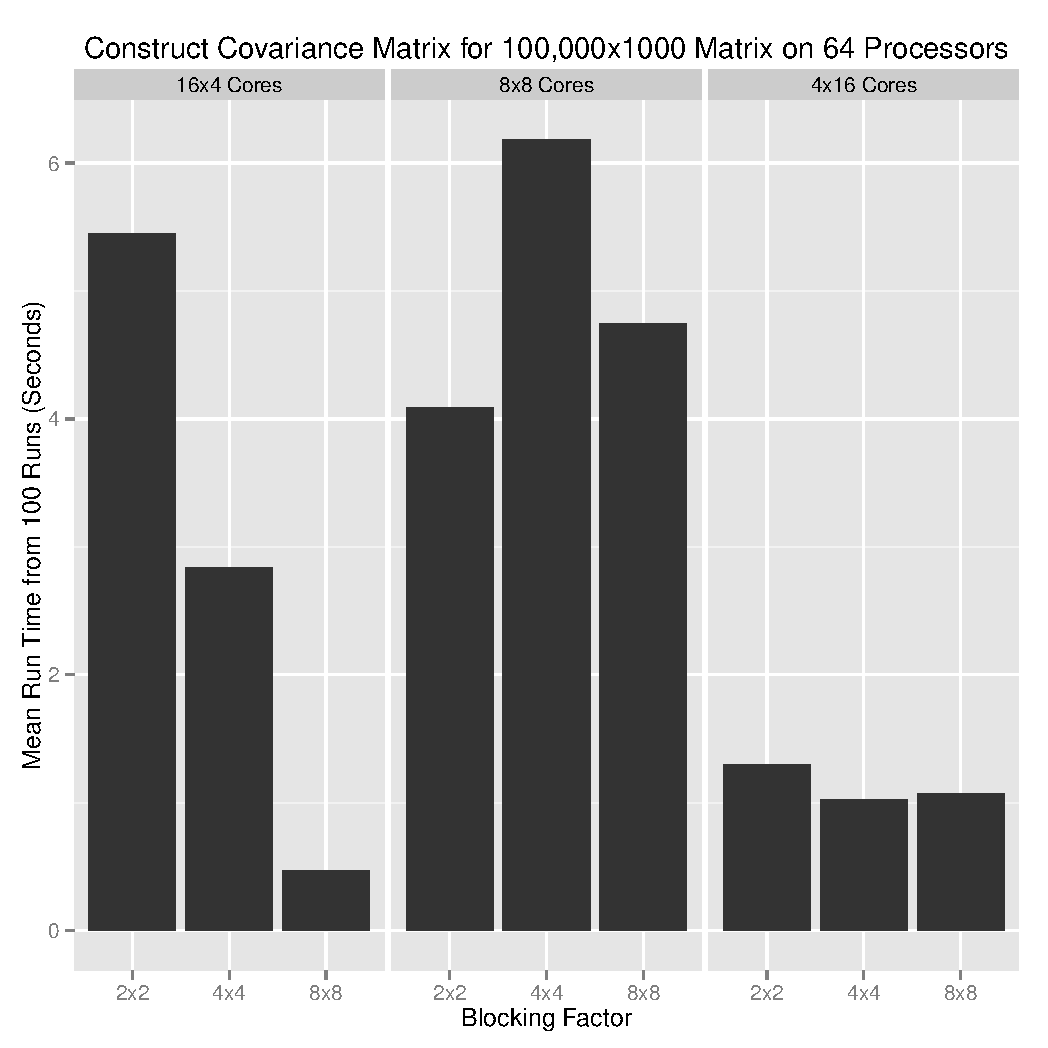
\includegraphics[width=10cm, height=7cm]{../common/pics/cov_param}
    \end{center}
  \end{block}
\end{frame}

\subsection{Future Work}

\begin{frame}
  \begin{block}{Future Work}
  \begin{itemize}
    \item Starting a 3 year NSF grant to work on
      \begin{itemize}
      \item Bring back interactivity via client/server
      \item Simplify parallel data input
      \item Begin DPLASMA integration
      \end{itemize}
    \item Optimization for heterogeneous architectures
    \item Support for more profilers
    \item In-situ use with simulations (QMC, AutoTune)
  \end{itemize}
  \end{block}
\end{frame}

\begin{frame}
  \begin{block}{Where to learn more?}
  \begin{itemize}
    \item \url{http://r-pbd.org/}
    \item \textbf{pbdDEMO} vignette
    \item \url{RBigData@gmail.com}
  \end{itemize}
  \end{block}
\end{frame}

